\documentclass[a4paper,12pt,oneside,English]{article}
\usepackage[a4paper,top=1.5cm,bottom=1.5cm,left=1cm,right=1cm]{geometry}
\usepackage[utf8]{inputenc}
\usepackage[T1]{fontenc}
\usepackage{blindtext}
\usepackage{framed}
\usepackage[svgnames]{xcolor}
\usepackage{graphicx}
\definecolor{shadecolor}{gray}{0.9}
\usepackage{mathtools}
\usepackage{caption}
\usepackage{subcaption}
\usepackage{dsfont}
\usepackage{nccmath}
\usepackage{graphicx}
\usepackage{amsthm}
\usepackage{color} 
\usepackage[pdftex,backref,linktocpage,colorlinks]{hyperref}
\usepackage{xcolor}
\usepackage{empheq}
\usepackage{adjustbox}
\usepackage{graphicx}
\usepackage{amssymb}
\usepackage{amsmath}
\usepackage{siunitx}
\usepackage{framed}
\usepackage{graphicx}
\documentclass[xcolor=table]{beamer}
\usepackage[table,xcdraw]{xcolor}
\usepackage[authoryear]{natbib}
\hypersetup{
    colorlinks,
    linkcolor={red!50!black},
    citecolor={red!50!black},
    urlcolor={red!50!black}
}
\usepackage{titling}
\usepackage{fancyhdr}
\usepackage[shortlabels]{enumitem}
\usepackage{float}
\usepackage[nottoc, notlof]{tocbibind}
\usepackage{setspace}
\usepackage[T1]{fontenc}
\usepackage{amsfonts}
\usepackage{amsmath}
\usepackage{indentfirst}
\renewcommand{\baselinestretch}{1.5}
\setlength{\skip\footins}{5ex plus 4pt minus 2pt}
\usepackage{rotating}
\usepackage{tocloft}
\setlength{\cftaftertoctitleskip}{1cm}
\setlength{\cftafterloftitleskip}{1cm}
\usepackage{enumitem}
\usepackage{titletoc,tocloft}
\setlength{\cftsubsecindent}{0cm}
\usepackage{floatflt} 
 \usepackage[bf, small]{caption}
 \usepackage[justification=centering]{caption}
 \setcounter{secnumdepth}{0}
\title{Problem Set 2 - Econometrics}
\author{ Giacomo Lo Conte, Kun Wu, Francesca Eustacchi, Neeharika Kakunuri, Noor Ahmed Khoso }

\begin{document}

\maketitle
\section{1. Theory}
\textbf{a. Consider a case where $Z$ is a binary instrument, $T$ is a discrete multi-valued treatment $(TZ \in {0,1,2,...,J})$, $T = Z T_1 + (1 − Z)T_0$ is the observed level of treatment, and $Y$ is the outcome. Assume that the random variables $T_0, T_1, Y_0, Y_1, . . . , Y_J$ are jointly independent of $J$ and that the level of treatment is higher when $Z = 1$ than when $Z = 0$, i.e. $T_1 − T_0 \geq 0$. Further, assume that $Pr(T_1 \geq j \geq T_0) > 0$ for at least one $j \in {0,1,2,...J}$, which means that the instrument on average affects the level of treatment. Show that under these assumptions the Wald estimator is a weighted average of the causal response of a unit change in treatment,
\begin{equation}
    \cfrac{E[Y| Z = 1] - E[Y | Z = 0]}{E[T| Z = 1] - E[T| Z = 0]} = \Sigma^J{j_=_1} w_j • E[Y_j - Y_j_1|T_1 \geq j > T_0],
\end{equation}
where the weight are 
\begin{equation}
w_j = \cfrac{Pr(T_1\geq j > T_0)}{\Sigma^J {_i_=_1}Pr(T_1\geq i > T_0)}
\end{equation}
b) Provide an interpretation of both factors on the RHS if Equation (1), i.e . $E [Y_j − Y_j−1 | T1 \geq j > T_0]$
and ωj. What does the presence of both factors teach us about the local average treatment effect?\\
c) In the lecture we have proven that in absence of defiers the IV estimate for an outcome $Y_i$, a binary treatment $D_i$ and a binary instrument $Z_i$ is
\begin{equation}
    \beta^IV∗ = E(Y_i|D_i = 1) − E(Y_i|D_i = 0)) = E(Y_i_1 − Y_i_0|complier)
\end{equation}
Now suppose the share of defiers is $0 < \phi D < 1$.
i) Derive the IV estimate for this case.
ii) Assume that $\phi D = a × \phi C with 0 < a < 1 and \beta^IV∗ > 0$. Discuss whether additional, plausible assumptions on $E(Y_i_1 − Y_i_0|defier)$ allow you to recover a lower bound for $\beta^IV∗$.}
\newpage


\section{2. Simulation Exercise}

\textbf{An important property of the IV estimator is that it is biased in small samples but consistent. For this reason one should never write that an IV estimator is used to obtain unbiased estimates. We want to better understand the small sample properties through simulations of the sampling distribution of IV and OLS estimators. In all simulations, let x, y, z, u and ε be random variables and assume the data-generating process:}

\begin{equation}
    y = \alpha+\beta x+ \epsilon
\end{equation}

\begin{equation}
    x = \gamma_0+\gamma_1z+ u
\end{equation}

\textbf{Set the parameter $\beta = 1$ and, unless required otherwise, $\alpha = \gamma_0 = 0$. Moreover, construct $\epsilon$ such that it's Pearson correlation with \textit{x} is 0.4.}


\subsection{a) Sampling Distribution under strong instruments}

\textbf{Construct the instrument $z$ such that its Pearson correlation with \textit{x} is 0.5 while its correlation with $\epsilon$ is zero. Consider four different sample sizes: $N = 50$, $N = 100$, $N = 250$ and $N = 1000$. For each sample size, run at least 10,000 simulations whereby you estimate $\beta^{OLS}$ and $\beta^{IV}$ (choose fewer replications if you have problems with computing power). In the same graph, plot the sampling distributions for OLS and IV for all four sample sizes. Discuss the difference in shape of the sampling distributions between OLS and IV.}

We constructed $x$, $z$ and $\epsilon$ through a random extraction of 10,000 observations. The three variable are correlated as required. Notice that, once we defined these three, the value of $\gamma_1$ can be defined as $\rho_{xz}\cfrac{\sigma_x}{\sigma_z}$. Its value then is defined by the ratio of the standard deviations, that are$\sigma_x=\sigma_z=\sigma_\epsilon=1$. In the second step, we derive $y=x+\epsilon$.

Among our population of 10,000 of units, we run a bootstrap (10,000 iterations) of our OLS and IV estimates over four different samples.
Graphics in figure \ref{Cor50} show clearly how the distributions of the the IV and OLS estimates change when the sample size increases.

\begin{figure}[p!]
    \begin{minipage}[b]{0.5\linewidth}
        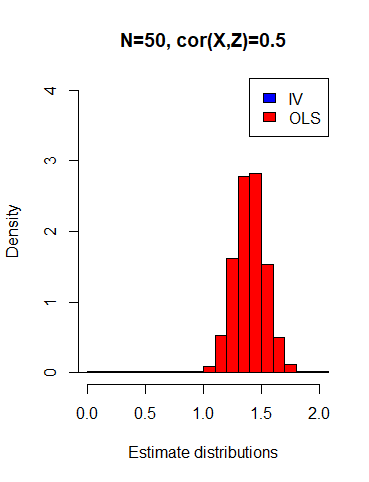
\includegraphics[width=\linewidth]{Fig1.png}
    \end{minipage}
    \begin{minipage}[b]{0.5\linewidth}
        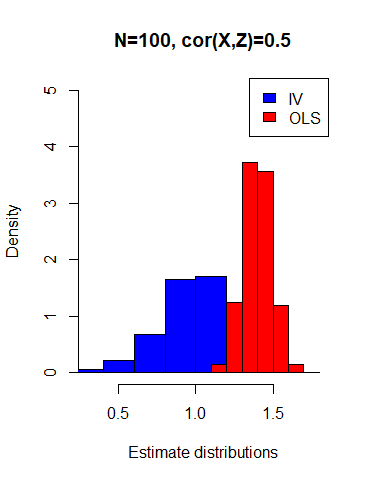
\includegraphics[width=\linewidth]{Fig2.png}
    \end{minipage}
    \begin{minipage}[b]{0.5\linewidth}
        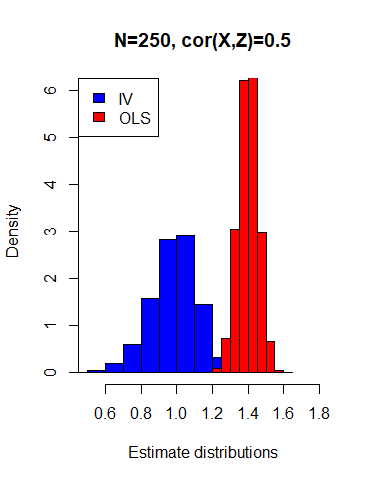
\includegraphics[width=\linewidth]{Fig3.png}
    \end{minipage}
    \begin{minipage}[b]{0.5\linewidth}
        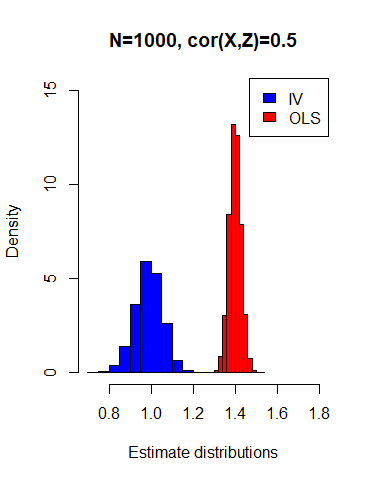
\includegraphics[width=\linewidth]{Fig4.png}
    \end{minipage}\hfill
    \label{Cor50}
    \caption{Distributions of IV and OLS estimates when $\rho_{XZ}=0.5$}
\end{figure}

How we can see, as long as the sample size increases we see that the distribution variance decreases both for the OLS and IV estimator. This is the graphic representation of the consistency property. Moreover, we can see graphically also the demonstration of the efficiency property of the OLS. OLS indeed shows a consistent lower variance and the frequency of the median values rises faster. In other words, IV estimator distribution is flatter than the OLS one. However, it is evident that OLS distribution biased, contrary to the IV. Indeed, while the IV estimator distribution is centered on 1, the OLS distribution is centered around 1.4. The bias is positive and is exactly equal to $\cfrac{Cov(x,\epsilon)}{\sigma^2_x}$. Since $Cov(x,\epsilon)=\rho_{x\epsilon}\sigma_x$, the bias is equal to $\cfrac{\rho_{x\epsilon}}{\sigma_x}\approx 0.4$. From these graphs, then it is clear that, in a non-biased setting the IV estimates may have more problems with the statistical inference. The IV errors are indeed larger than the OLS.

\subsection{b) Weaker instruments:}
\textbf{Now repeat the analysis from a), but instead assume that the correlation between the instrument $z$ and the regressor $x$ is $0.15$. Discuss the difference in sampling distributions between OLS and IV and, in addition, discuss the difference between sampling distributions based on weak and strong IVs.}

\begin{figure}[p!]
    \begin{minipage}[b]{0.5\linewidth}
        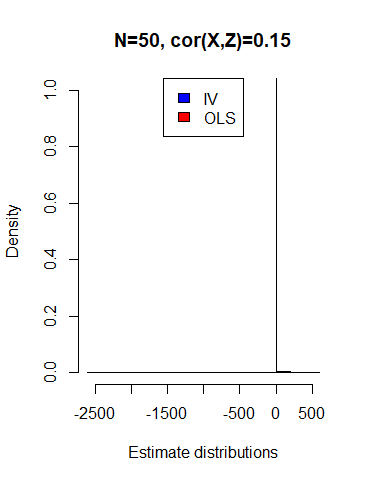
\includegraphics[width=\linewidth]{Fig1A.png}
    \end{minipage}
    \begin{minipage}[b]{0.5\linewidth}
        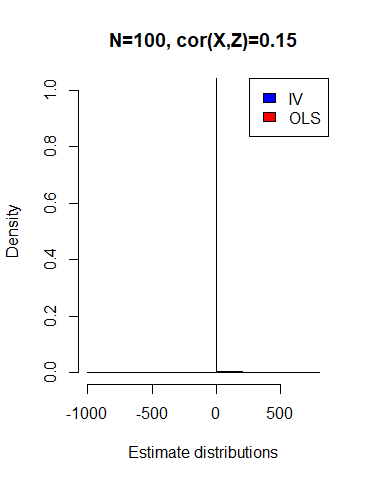
\includegraphics[width=\linewidth]{Fig2A.png}
    \end{minipage}
    \begin{minipage}[b]{0.5\linewidth}
        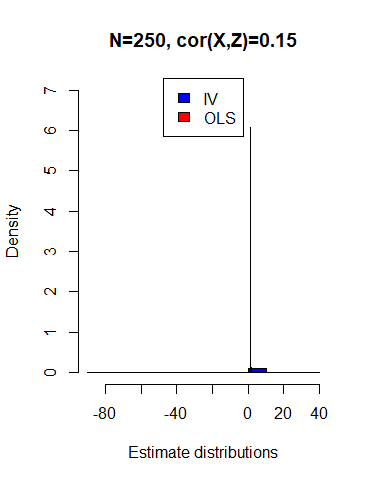
\includegraphics[width=\linewidth]{Fig3A.png}
    \end{minipage}
    \begin{minipage}[b]{0.5\linewidth}
        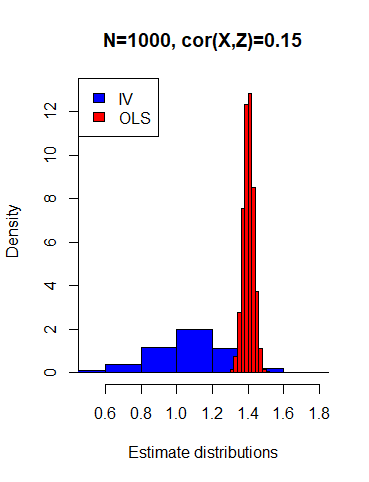
\includegraphics[width=\linewidth]{Fig4A.png}
    \end{minipage}\hfill
    \label{cor15}
    \caption{Distributions of IV and OLS estimates when $\rho_{XZ}=0.15$}
\end{figure}

In figure \ref{cor15} we can hardly observe the OLS distribution for a problem of scale, however it remains basically unchanged. In the IV case, we can notice a very different scenario. The IV distribution is much flatter than the previous case. To fully grasp the difference we can observe the scale of the axes. While in figure \ref{Cor50}, the top-right graph presents an interval between 0.3 and 1.7, in figure \ref{cor15} the same graph the interval is between -1000 and 600. This is due to the formula of the variance for the IV estimator. The asymptotic variance of the IV is:
\[
\widehat{Avar}(\beta^{IV}-\beta|X,Z)=E[(Z'X)^{-1}Z'uu'Z(Z'X)^{-1}|X,Z]
\]
\[
\widehat{Avar}(\beta^{IV}-\beta)=E[uu'](Z'X)^{-1}=\Sigma^2_u(Z'X)^{-1}
\]
The asymptotic variance of the IV estimator can be written as the variance matrix of the error times the inverse of the covariance of Z and X. In our simple univariate case $Z'X=Cov(x,z)=\rho_{xz}\sigma_z\sigma_x$=. The variance of the estimator, then, is inversely related to $\rho_{xz}$. For this reason, the weaker is the instrument and the higher is the variance of the IV estimator. This leads to problems for the statistical inference since the results are not significant even if unbiased.

\newpage
\section{Empirical Application}

The empirical application is based on a cross-sectional dataset assign2.dta, which contains the following variables:
\begin{itemize}
    \item \textit{age}: age of surveyed individual
    \item \textit{logearn}: log annual earnings
    \item \textit{yob}: year of birth
    \item \textit{schooling}: age at which the person left school.
\end{itemize}
a) The goal is to estimate the returns to education. For this purpose, estimate an OLS regression of \textit{logearn} on schooling, controlling for fourth-order polynomials in age and year of birth. Interpret the coeffcient of schooling.
A common way to obtain causal estimates is to use changes in compulsory schooling laws for identification. In this case, birth cohorts born before 1933 $(yob<33)$ had to go to school until they were 14 years old, whereas compulsory schooling age was raised to 15 years for all cohorts born from 1933 onwards. This change in compulsory schooling laws can be used as an instrumental variable for the actual duration of schooling. The instrument is a dummy LAW that equals unity if a person is born 1933 or later and zero otherwise.

Benchmark regression :
\begin{table}[!htbp] \centering 
  \caption{Benchmark Regression - tbd} 
  \label{reg 1} 
\begin{tabular}{@{\extracolsep{5pt}}lc} 
\\[-1.8ex]\hline 
\hline \\[-1.8ex] 
 & \multicolumn{1}{c}{\textit{Dependent variable:}} \\ 
\cline{2-2} 
\\[-1.8ex] & logearn \\ 
\hline \\[-1.8ex] 
 age & 0.005$^{***}$ \\ 
  & (0.001) \\ 
  & \\ 
 yob & 0.005$^{***}$ \\ 
  & (0.001) \\ 
  & \\ 
 schooling & 0.157$^{***}$ \\ 
  & (0.002) \\ 
  & \\ 
 Constant & 2.964$^{***}$ \\ 
  & (0.055) \\ 
  & \\ 
\hline \\[-1.8ex] 
Observations & 30,801 \\ 
R$^{2}$ & 0.140 \\ 
Adjusted R$^{2}$ & 0.140 \\ 
Residual Std. Error & 0.496 (df = 30797) \\ 
F Statistic & 1,673.896$^{***}$ (df = 3; 30797) \\ 
\hline 
\hline \\[-1.8ex] 
\textit{Note:}  & \multicolumn{1}{r}{$^{*}$p$<$0.1; $^{**}$p$<$0.05; $^{***}$p$<$0.01} \\ 
\end{tabular} 
\end{table}

\begin{table}[!htbp] \centering 
  \caption{Regression with the 4th order polynomial for age and year of birth} 
  \label{reg 2} 
\begin{tabular}{@{\extracolsep{5pt}}lc} 
\\[-1.8ex]\hline 
\hline \\[-1.8ex] 
 & \multicolumn{1}{c}{\textit{Dependent variable:}} \\ 
\cline{2-2} 
\\[-1.8ex] & logearn \\ 
\hline \\[-1.8ex] 
 age & 0.005$^{***}$ \\ 
  & (0.001) \\ 
  & \\ 
 yob & 0.005$^{***}$ \\ 
  & (0.001) \\ 
  & \\ 
 schooling & 0.157$^{***}$ \\ 
  & (0.002) \\ 
  & \\ 
 Constant & 2.964$^{***}$ \\ 
  & (0.055) \\ 
  & \\ 
\hline \\[-1.8ex] 
Observations & 30,801 \\ 
R$^{2}$ & 0.140 \\ 
Adjusted R$^{2}$ & 0.140 \\ 
Residual Std. Error & 0.496 (df = 30797) \\ 
F Statistic & 1,673.896$^{***}$ (df = 3; 30797) \\ 
\hline 
\hline \\[-1.8ex] 
\textit{Note:}  & \multicolumn{1}{r}{$^{*}$p$<$0.1; $^{**}$p$<$0.05; $^{***}$p$<$0.01} \\ 
\end{tabular} 
\end{table} 
b) Discuss this instrument in theory, assuming that schooling Si is related to the instrument $Z_i$ by the latent assignment mechanism
\begin{equation*}
    S_i = 1(\gamma_0+ \gamma_1 Z_i > \eta_i),\;\; with\;\; E(Z_i \eta _i) = 0
\end{equation*}
The random variable ηi represents the individual resistance to treatment. Why could there be a
first stage? Under what condition is this instrument valid? What are potential threats to validity?
 2
Furthermore, explain who are the compliers, always-takers and never-takers in this case. Would the IV estimate correspond to the average treatment effect (why or why not)?
c) As in any good empirical project, begin with a graphical inspection of the relationships of interest. This is best done through binscatters. Produce and discuss the graphs listed below. In all graphs, include a vertical line at $yob=33$.
\begin{itemize}
    \item Plot the probability that a person leaves school before age 15 against the year of birth.
    \item Binscatter of schooling and year of birth
    \item Binscatter of log earnings and year of birth.
\end{itemize}
d) Calculate the Wald estimator (without controls) "by hand", i.e. based on conditional averages. Compare your results to those of a 2SLS estimation based on an inbuilt command (e.g. \textit{ivregress} in Stata or \textit{ivreg} in R). Interpret your results and compare them to the OLS results in a).
\begin{table}[!htbp] \centering 
  \caption{Regression of D on Z } 
  \label{reg 3} 
\begin{tabular}{@{\extracolsep{5pt}}lc} 
\\[-1.8ex]\hline 
\hline \\[-1.8ex] 
 & \multicolumn{1}{c}{\textit{Dependent variable:}} \\ 
\cline{2-2} 
\\[-1.8ex] & schooling \\ 
\hline \\[-1.8ex] 
 LAW & 0.990$^{***}$ \\ 
  & (0.014) \\ 
  & \\ 
 Constant & 14.624$^{***}$ \\ 
  & (0.012) \\ 
  & \\ 
\hline \\[-1.8ex] 
Observations & 30,801 \\ 
R$^{2}$ & 0.137 \\ 
Adjusted R$^{2}$ & 0.136 \\ 
Residual Std. Error & 1.146 (df = 30799) \\ 
F Statistic & 4,868.939$^{***}$ (df = 1; 30799) \\ 
\hline 
\hline \\[-1.8ex] 
\textit{Note:}  & \multicolumn{1}{r}{$^{*}$p$<$0.1; $^{**}$p$<$0.05; $^{***}$p$<$0.01} \\ 
\end{tabular} 
\end{table} 

\begin{table}[!htbp] \centering 
  \caption{Regression of Y on Z} 
  \label{reg 4} 
\begin{tabular}{@{\extracolsep{5pt}}lc} 
\\[-1.8ex]\hline 
\hline \\[-1.8ex] 
 & \multicolumn{1}{c}{\textit{Dependent variable:}} \\ 
\cline{2-2} 
\\[-1.8ex] & logearn \\ 
\hline \\[-1.8ex] 
 LAW & 0.162$^{***}$ \\ 
  & (0.007) \\ 
  & \\ 
 Constant & 5.671$^{***}$ \\ 
  & (0.005) \\ 
  & \\ 
\hline \\[-1.8ex] 
Observations & 30,801 \\ 
R$^{2}$ & 0.019 \\ 
Adjusted R$^{2}$ & 0.019 \\ 
Residual Std. Error & 0.530 (df = 30799) \\ 
F Statistic & 607.678$^{***}$ (df = 1; 30799) \\ 
\hline 
\hline \\[-1.8ex] 
\textit{Note:}  & \multicolumn{1}{r}{$^{*}$p$<$0.1; $^{**}$p$<$0.05; $^{***}$p$<$0.01} \\ 
\end{tabular} 
\end{table} 
The manual Wald estimator is 0.1633267.

\begin{table}[!htbp] \centering 
  \caption{IVREG with R code} 
  \label{reg 5} 
\begin{tabular}{@{\extracolsep{5pt}}lc} 
\\[-1.8ex]\hline 
\hline \\[-1.8ex] 
 & \multicolumn{1}{c}{\textit{Dependent variable:}} \\ 
\cline{2-2} 
\\[-1.8ex] & logearn \\ 
\hline \\[-1.8ex] 
 schooling & 0.163$^{***}$ \\ 
  & (0.006) \\ 
  & \\ 
 Constant & 3.283$^{***}$ \\ 
  & (0.095) \\ 
  & \\ 
\hline \\[-1.8ex] 
Observations & 30,801 \\ 
R$^{2}$ & 0.138 \\ 
Adjusted R$^{2}$ & 0.138 \\ 
Residual Std. Error & 0.497 (df = 30799) \\ 
\hline 
\hline \\[-1.8ex] 
\textit{Note:}  & \multicolumn{1}{r}{$^{*}$p$<$0.1; $^{**}$p$<$0.05; $^{***}$p$<$0.01} \\ 
\end{tabular} 
\end{table} 
\end{document}
